%% This file was auto-generated by IPython.
%% Conversion from the original notebook file:
%% knn2.ipynb
%%
\documentclass[11pt,english,fleqn]{article}

%% This is the automatic preamble used by IPython.  Note that it does *not*
%% include a documentclass declaration, that is added at runtime to the overall
%% document.

\usepackage{amsmath}
\usepackage{amssymb}
\usepackage{graphicx}
\usepackage{ucs}
\usepackage[utf8x]{inputenc}

% needed for markdown enumerations to work
\usepackage{enumerate}

% Slightly bigger margins than the latex defaults
\usepackage{geometry}
\geometry{verbose,tmargin=3cm,bmargin=3cm,lmargin=2.5cm,rmargin=2.5cm}

% Define a few colors for use in code, links and cell shading
\usepackage{color}
\definecolor{orange}{cmyk}{0,0.4,0.8,0.2}
\definecolor{darkorange}{rgb}{.71,0.21,0.01}
\definecolor{darkgreen}{rgb}{.12,.54,.11}
\definecolor{myteal}{rgb}{.26, .44, .56}
\definecolor{gray}{gray}{0.45}
\definecolor{lightgray}{gray}{.95}
\definecolor{mediumgray}{gray}{.8}
\definecolor{inputbackground}{rgb}{.95, .95, .85}
\definecolor{outputbackground}{rgb}{.95, .95, .95}
\definecolor{traceback}{rgb}{1, .95, .95}

% Framed environments for code cells (inputs, outputs, errors, ...).  The
% various uses of \unskip (or not) at the end were fine-tuned by hand, so don't
% randomly change them unless you're sure of the effect it will have.
\usepackage{framed}

% remove extraneous vertical space in boxes
\setlength\fboxsep{0pt}

% codecell is the whole input+output set of blocks that a Code cell can
% generate.

% TODO: unfortunately, it seems that using a framed codecell environment breaks
% the ability of the frames inside of it to be broken across pages.  This
% causes at least the problem of having lots of empty space at the bottom of
% pages as new frames are moved to the next page, and if a single frame is too
% long to fit on a page, will completely stop latex from compiling the
% document.  So unless we figure out a solution to this, we'll have to instead
% leave the codecell env. as empty.  I'm keeping the original codecell
% definition here (a thin vertical bar) for reference, in case we find a
% solution to the page break issue.

%% \newenvironment{codecell}{%
%%     \def\FrameCommand{\color{mediumgray} \vrule width 1pt \hspace{5pt}}%
%%    \MakeFramed{\vspace{-0.5em}}}
%%  {\unskip\endMakeFramed}

% For now, make this a no-op...
\newenvironment{codecell}{}

 \newenvironment{codeinput}{%
   \def\FrameCommand{\colorbox{inputbackground}}%
   \MakeFramed{\advance\hsize-\width \FrameRestore}}
 {\unskip\endMakeFramed}

\newenvironment{codeoutput}{%
   \def\FrameCommand{\colorbox{outputbackground}}%
   \vspace{-1.4em}
   \MakeFramed{\advance\hsize-\width \FrameRestore}}
 {\unskip\medskip\endMakeFramed}

\newenvironment{traceback}{%
   \def\FrameCommand{\colorbox{traceback}}%
   \MakeFramed{\advance\hsize-\width \FrameRestore}}
 {\endMakeFramed}

% Use and configure listings package for nicely formatted code
\usepackage{listingsutf8}
\lstset{
  language=python,
  inputencoding=utf8x,
  extendedchars=\true,
  aboveskip=\smallskipamount,
  belowskip=\smallskipamount,
  xleftmargin=2mm,
  breaklines=true,
  basicstyle=\small \ttfamily,
  showstringspaces=false,
  keywordstyle=\color{blue}\bfseries,
  commentstyle=\color{myteal},
  stringstyle=\color{darkgreen},
  identifierstyle=\color{darkorange},
  columns=fullflexible,  % tighter character kerning, like verb
}

% The hyperref package gives us a pdf with properly built
% internal navigation ('pdf bookmarks' for the table of contents,
% internal cross-reference links, web links for URLs, etc.)
\usepackage{hyperref}
\hypersetup{
  breaklinks=true,  % so long urls are correctly broken across lines
  colorlinks=true,
  urlcolor=blue,
  linkcolor=darkorange,
  citecolor=darkgreen,
  }

% hardcode size of all verbatim environments to be a bit smaller
\makeatletter 
\g@addto@macro\@verbatim\small\topsep=0.5em\partopsep=0pt
\makeatother 

% Prevent overflowing lines due to urls and other hard-to-break entities.
\sloppy

\setlength{\mathindent}{0pt}
\setlength{\parindent}{0pt}
\setlength{\parskip}{8pt}
\begin{document}

En Yakin k-Komsu (k-Nearest Neighbor)

Yapay Ogrenim alaninda ornek bazli ogrenen algoritmalardan bilinen kNN,
egitim verinin kendisini siniflama (classification) amacli olarak
kullanir, yeni bir model ortaya cikartmaz. Algoritma soyle isler:
etiketleri bilinen egitim verisi alinir ve bir kenarda tutulur. Yeni bir
veri noktasi xqgorulunce bu veriye geri donulur ve o noktaya ``en
yakin'' k tane nokta bulunur. Daha sonra bu noktalarin etiketlerine
bakilir ve cogunlugun etiketi ne ise, o etiket yeni noktanin etiketi
olarak kabul edilir. Mesela elde 1 kategorisi altinda {[}2 2{]}, 2
kategorisi altinda {[}5 5{]} var ise, yeni nokta {[}3, 3{]} icin
yakinlik acisindan {[}2 2{]} bulunmali ve etiket olarak 1 sonucu
dondurulmelidir.

Ustte tarif edilen basit bir ihtiyac, yontem gibi gorulebilir. Fakat
yapay ogrenim ve yapay zeka cok boyutlarda oruntu tanima (pattern
recognition) ile ugrasir, ve milyonlarca satirlik veri, onlarca boyut
(ustteki ornekte 2, fakat cogunlukla cok daha fazla boyut vardir) isler
hakikaten zorlasabilir. Mesela goruntu tanimada veri M x N boyutundaki
dijital imajlar (duzlestirilince $M \cdot N$ boyutunda), ve onlarin
icindeki resimlerin kime ait oldugu etiket bilgisi olabilir. kNN bu tur
multimedya, cok boyutlu veri ortaminda basarili sekilde
calisabilmektedir. Ayrica en yakin k komsunun icerigi tarifsel bilgi
cikarimi (knowledge extraction) amaciyla da kullanilabilir {[}2{]}.

``En yakin'' sozu bir kordinat sistemi anlamina geliyor, ve kNN, aynen
k-Means ve diger pek cok kordinatsal ogrenme yontemi gibi eldeki cok
boyutlu veri noktalarinin elemanlarini bir kordinat sistemindeymis gibi
gorur. Kiyasla mesela APriori gibi bir algoritma metin bazli veriyle
oldugu gibi calisabilirdi.

Peki arama baglaminda, bir veri obegi icinden en yakin noktalari
bulmanin en basit yolu nedir? Listeyi bastan sonra taramak (kaba kuvvet
yontemi -brute force-) listedeki her nokta ile yeni nokta arasindaki
mesafeyi teker teker hesaplayip en yakin k taneyi icinden secerdi, bu
bir yontemdir.. Bu basit algoritmanin yuku $O(N)$'dir. Eger tek bir
nokta ariyor olsaydik, kabul edilebilir olabilirdi. Fakat genellikle bir
siniflayici (classifier) algoritmasinin surekli islemesi, mesela bir
online site icin gunde milyonlarca kez bazi kararlari almasi
gerekebilir. Bu durumda ve $N$'in cok buyuk oldugu sartlarda, ustteki
hiz bile yeterli olmayacaktir.

Arama islemini daha hizli yapmanin yollari var. Akilli arama
algoritmalari kullanarak egitim verilerini bir agac yapisi uzerinden
tarayip erisim hizini $O(\log N)$'e indirmek mumkundur.

Küre Agaçları (Ball Tree, BT)

Bir noktanin diger noktalara yakin olup olmadiginin hesabinda yapilmasi
gereken en pahali islem nedir? Mesafe hesabidir. BT algoritmasinin puf
noktasi bu hesabi yapmadan, noktalara degil, noktalari kapsayan
``kurelere'' bakarak hiz kazandirmasidir. Noktalarin her biri yerine o
noktalari temsil eden kurenin mihenk noktasina (pivot -bu nokta kure
icindeki noktalarin ortalamasal olarak merkezi de olabilir, herhangi bir
baska nokta da-) bakilir, ve oraya olan mesafeye gore bir kure altindaki
noktalara olabilecek en az ve en fazla uzaklik hemen anlasilmis olur.

Not: Kure kavrami uc boyutta anlamli tabii ki, iki boyutta bir cemberden
bahsetmek lazim, daha yuksek boyutlarda ise merkezi ve capi olan bir
``hiper yuzeyden'' bahsetmek lazim. Tarifi kolaylastirdigi icin cember
ve kure tanimlarini kullaniyoruz.

Mesela elimizde alttaki gibi noktalar var ve kureyi olusturduk.

\begin{codecell}
\begin{codeinput}
\begin{lstlisting}
im=imread("knn0.png"); imshow(im)
\end{lstlisting}
\end{codeinput}
\begin{codeoutput}
\begin{verbatim}
<matplotlib.image.AxesImage at 0xc204f0c>
\end{verbatim}
\begin{center}
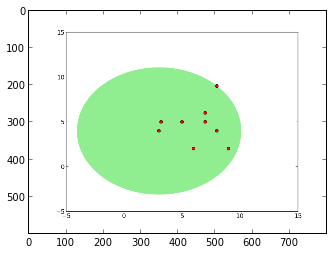
\includegraphics[width=0.7\textwidth]{knn2_files/knn2_fig_00.png}
\par
\end{center}
\end{codeoutput}
\end{codecell}
Bu kureyi kullanarak kure disindaki herhangi bir nokta $q$'nun kuredeki
``diger tum noktalar $x$'e'' olabilecegi en az mesafenin ne olacagini
ucgensel esitsizlik ile anlayabiliriz.

Ucgensel esitsizlik
\[ |x-y| \le |x-z| + |z-y| \]
$||$ operatoru norm operatoru anlamina gelir ve uzaklik hesabinin
genellestirilmis halidir. Konu hakkinda daha fazla detay icin
\emph{Fonksinel Analiz} ders notlarimiza bakabilirsiniz. Kisaca
soylenmek istenen iki nokta arasinda direk gitmek yerine yolu uzatirsak,
mesafe artacagidir. Tabii uzaklik, yol, nokta gibi kavramlar tamamen
soyut matematiksel ortamda da isleyecek sekilde ayarlanmistir. Mesela
mesafe (norm) kavramini degistirebiliriz, Oklitsel yerine Manhattan
mesafesi kullaniriz, fakat bu kavram bir norm oldugu ve belirttigimiz
uzayda gecerli oldugu icin ucgensel esitsizlik uzerine kurulmus tum
diger kurallar gecerli olur.

\begin{codecell}
\begin{codeinput}
\begin{lstlisting}
im=imread("tri1.png"); imshow(im)

\end{lstlisting}
\end{codeinput}
\begin{codeoutput}
\begin{verbatim}
<matplotlib.image.AxesImage at 0xc37f6cc>
\end{verbatim}
\begin{center}
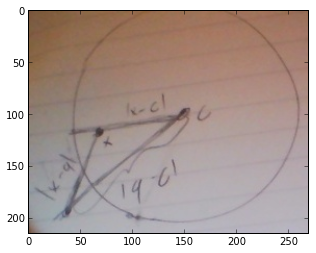
\includegraphics[width=0.7\textwidth]{knn2_files/knn2_fig_01.png}
\par
\end{center}
\end{codeoutput}
\end{codecell}
Simdi diyelim ki disaridaki bir $q$ noktasindan bir kure icindeki diger
tum $x$ noktalarina olan mesafe hakkinda bir seyler soylemek istiyoruz.
Ustteki sekilden bir ucgensel esitsizlik cikartabiliriz,
\[ |x-c| + |x-q| \ge |q-c|  \]
Bunun dogru bir ifade oldugunu biliyoruz. Peki simdi yaricapi bu ise
dahil edelim, cunku yaricap hesabi bir kere yapilip kure seviyesinde
depolanacak ve bir daha hesaplanmasi gerekmeyecek, yani algoritmayi
hizlandiracak bir sey olabilir bu, o zaman eger $|x-c|$ yerine yaricapi
kullanirsak, esitsizlik hala gecerli olur, sol taraf zaten buyuktu,
simdi daha da buyuk olacak,
\[ radius + |x-q| \ge |q-c|  \]
Bunu nasil boyle kesin bilebiliyoruz? Cunku BT algoritmasi radius'u
$|x-c|$'ten kesinlikle daha buyuk olacak sekilde secer). Simdi yaricapi
saga gecirelim,
\[ |x-q| \ge |q-c| - radius \]
Boylece guzel bir tanim elde ettik. Yeni noktanin kuredeki herhangi bir
nokta $x$'e olan uzakligi, yeni noktanin mihenke olan uzakliginin
yaricapi cikartilmis halinden \emph{muhakkak} fazladir. Yani bu cikartma
isleminden ele gecen rakam yeni noktanin $x$'e uzakligina bir ``alt
sinir (lower bound)'' olarak kabul edilebilir. Diger tum mesafeler bu
rakamdan daha buyuk olacaktir. Ne elde ettik? Sadece bir yeni nokta,
mihenk ve yaricap kullanarak kuredeki ``diger tum noktalar hakkinda''
bir irdeleme yapmamiz mumkun olacak. Bu noktalara teker teker bakmamiz
gerekmeyecek. Bunun nasil ise yaradigini algoritma detaylarinda
gorecegiz.

Benzer sekilde

\begin{codecell}
\begin{codeinput}
\begin{lstlisting}
im=imread("tri2.png"); imshow(im)
\end{lstlisting}
\end{codeinput}
\begin{codeoutput}
\begin{verbatim}
<matplotlib.image.AxesImage at 0xc4e49ac>
\end{verbatim}
\begin{center}
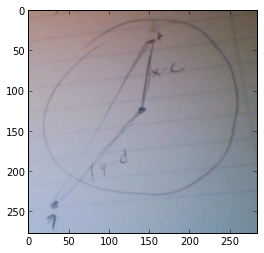
\includegraphics[width=0.7\textwidth]{knn2_files/knn2_fig_02.png}
\par
\end{center}
\end{codeoutput}
\end{codecell}
Bu ne diyor?
\[ |q-c| + |x-c| \ge |q-x| \]
$|x-c|$ yerine yaricap kullanirsak, sol taraf buyuyecegi icin buyukluk
hala buyukluk olarak kalir,
\[ |q-c| + radius \ge |q-x| \]
Ve yine daha genel ve hizli hesaplanan bir kural elde ettik (onceki
ifadeye benzemesi icin yer duzenlemesi yapalim)
\[ |q-x| \le |q-c| + radius \]
Bu ifade ne diyor? Yeni noktanin mihenke olan uzakligina yaricap
``eklenirse'' bu uzakliktan, buyuklukten daha buyuk bir yeni nokta /
kure mesafesi olamaz, kuredeki hangi nokta olursa olsun. Bu esitsizlik
te bize bir ust sinir (upper bound) vermis oldu.

Algoritma

Kure Agaclari (BT) metotu once kureleri, agaclari olusturmalidir. Bu
kureler hiyerarsik sekilde planlanir, tum noktalarin icinde oldugu bir
``en ust kure'' vardir her kurenin iki tane cocuk kuresi olabilir. Belli
bir (disaridan tanimlanan) minimum $r_{min}$ veri noktasina gelinceye
kadar sadece noktalari geometrik olarak kapsamakla goreli kureler
olusturulur, kureler noktalari sahiplenmezler. Fakat bu $r_{min}$
sayisina erisince (artik oldukca alttaki) kurelerin uzerine noktalar
konacaktir.

Once tek kurenin olusturulusuna bakalim. Bir kure olusumu icin eldeki
veri icinden herhangi bir tanesi mihenk olarak kabul edilebilir. Daha
sonra bu mihenkten diger tum noktalara olan uzaklik olculur, ve en
fazla, en buyuk olan uzaklik yaricap olarak kabul edilir (her seyi
kapsayabilmesi icin).

Not: Bu arada ``tum diger noktalara bakilmasi'' dedik, bundan kacinmaya
calismiyor muyduk? Fakat dikkat, ``kure olusturulmasi'' evresindeyiz, k
tane yakin nokta arama evresinde degiliz. Yapmaya calistigimiz aramalari
hizlandirmak - egitim / kure olusturmasi bir kez yapilacak ve bu
egitilmis kureler bir kenarda tutulacak ve surekli aramalar icin ardi
ardina kullanilacaklar.

Kureyi olusturmanin algoritmasi soyledir: verilen noktalar icinde
herhangi birisi mihenk olarak secilir. Sonra bu noktadan en uzakta olan
nokta $f_1$, sonra $f_1$'den en uzakta olan nokta $f_2$ secilir. Sonra
tum noktalara teker teker bakilir ve $f_1$'e yakin olanlar bir gruba,
$f_2$'ye yakin olanlar bir gruba ayrilir.

\begin{codecell}
\begin{codeinput}
\begin{lstlisting}
import itertools

def dist(vect,x):
    return np.fromiter(itertools.imap
                       (np.linalg.norm, vect-x),dtype=np.float)

def norm(x,y): return np.linalg.norm(x-y)

# small test
points = np.array([[3.,3.],[2.,2.]])
q = [1.,1.]
print "diff", points-q
print "dist", dist(points,q)

\end{lstlisting}
\end{codeinput}
\begin{codeoutput}
\begin{verbatim}
diff [[ 2.  2.]
 [ 1.  1.]]
dist [ 2.82842712  1.41421356]
\end{verbatim}
\end{codeoutput}
\end{codecell}
\begin{codecell}
\begin{codeinput}
\begin{lstlisting}
#
# k-nearest neighbor Ball Tree algorithm in Python
#
import pprint
import numpy as np

__rmin__ = 2

# node: [pivot, radius, points, [child1,child2]]
def new_node(): return  [None,None,None,[None,None]]

def zero_if_neg(x):
    if x < 0: return 0
    else: return x

def form_tree(points,node):    
    pivot = points[0]
    radius = np.max(dist(points,pivot))
    node[0] = pivot
    node[1] = radius
    if len(points) <= __rmin__:
        node[2] = points
        return
    idx = np.argmax(dist(points,pivot))
    furthest = points[idx,:]
    idx = np.argmax(dist(points,furthest))
    furthest2 = points[idx,:]
    dist1=dist(points,furthest)
    dist2=dist(points,furthest2)
    diffs = dist1-dist2
    p1 = points[diffs <= 0]
    p2 = points[diffs > 0]
    node[3][0] = new_node() # left child
    node[3][1] = new_node() # right child
    form_tree(p1,node[3][0])
    form_tree(p2,node[3][1])

# knn: [min_so_far, [points]]
def search_tree(new_point, knn_matches, node, k):
    pivot = node[0]
    radius = node[1]
    node_points = node[2]
    children = node[3]

    # calculate min distance between new point and pivot
    # it is direct distance minus the radius
    min_dist_new_pt_node = norm(pivot,new_point) - radius
    
    # if the new pt is inside the circle, its potential minimum
    # distance to a random point inside is zero (hence
    # zero_if_neg). we can only say so much without looking at all
    # points (and if we did, that would defeat the purpose of this
    # algorithm)
    min_dist_new_pt_node = zero_if_neg(min_dist_new_pt_node)
    
    knn_matches_out = None
    
    # min is greater than so far
    if min_dist_new_pt_node >= knn_matches[0]:
        # nothing to do
        return knn_matches
    elif node_points != None: # if node is a leaf
        print knn_matches_out
        knn_matches_out = knn_matches[:] # copy it
        for p in node_points: # linear scan
            if norm(new_point,p) < radius:
                knn_matches_out[1].append([list(p)])
                if len(knn_matches_out[1]) == k+1:
                    tmp = [norm(new_point,x) \
                               for x in knn_matches_out[1]]
                    del knn_matches_out[1][np.argmax(tmp)]
                    knn_matches_out[0] = np.min(tmp)

    else:
        dist_child_1 = norm(children[0][0],new_point)
        dist_child_2 = norm(children[1][0],new_point)
        node1 = None; node2 = None
        if dist_child_1 < dist_child_2:
            node1 = children[0]
            node2 = children[1]
        else:
            node1 = children[1]
            node2 = children[0]

        knn_tmp = search_tree(new_point, knn_matches, node1, k)
        knn_matches_out = search_tree(new_point, knn_tmp, node2, k)
            
    return knn_matches_out
                   
points = np.array([[3.,4.],[5.,5.],[9.,2.],[3.2,5.],[7.,5.],
                 [8.,9.],[7.,6.],[8,4],[6,2]])
tree = new_node()
form_tree(points,tree)
pp = pprint.PrettyPrinter(indent=4)
print "tree"
pp.pprint(tree)
newp = np.array([7.,7.])
dummyp = [np.Inf,np.Inf] # it should be removed immediately
res = search_tree(newp,[np.Inf, [dummyp]], tree, k=2)
print "done", res

\end{lstlisting}
\end{codeinput}
\begin{codeoutput}
\begin{verbatim}
tree
[   array([ 3.,  4.]),
    7.0710678118654755,
    None,
    [   [   array([ 8.,  9.]),
            3.1622776601683795,
            array([[ 8.,  9.],
       [ 7.,  6.]]),
            [None, None]],
        [   array([ 3.,  4.]),
            6.324555320336759,
            None,
            [   [   array([ 9.,  2.]),
                    3.6055512754639891,
                    None,
                    [   [   array([ 7.,  5.]),
                            1.4142135623730951,
                            array([[ 7.,  5.],
       [ 8.,  4.]]),
                            [None, None]],
                        [   array([ 9.,  2.]),
                            3.0,
                            array([[ 9.,  2.],
       [ 6.,  2.]]),
                            [None, None]]]],
                [   array([ 3.,  4.]),
                    2.2360679774997898,
                    None,
                    [   [   array([ 5.,  5.]),
                            0.0,
                            array([[ 5.,  5.]]),
                            [None, None]],
                        [   array([ 3.,  4.]),
                            1.019803902718557,
                            array([[ 3. ,  4. ],
       [ 3.2,  5. ]]),
                            [None, None]]]]]]]]
None
done [1.0, [[[8.0, 9.0]], [[7.0, 6.0]]]]
\end{verbatim}
\end{codeoutput}
\end{codecell}
\begin{codecell}
\begin{codeinput}
\begin{lstlisting}
im=imread("alg.png");imshow(im)
\end{lstlisting}
\end{codeinput}
\begin{codeoutput}
\begin{verbatim}
<matplotlib.image.AxesImage at 0xc67916c>
\end{verbatim}
\begin{center}
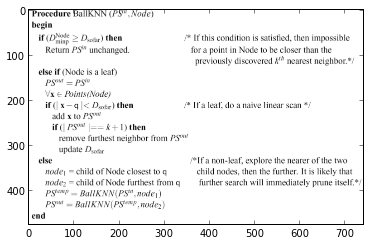
\includegraphics[width=0.7\textwidth]{knn2_files/knn2_fig_03.png}
\par
\end{center}
\end{codeoutput}
\end{codecell}
Bu iki grup, o anda islemekte oldugumuz agac dugumun (node) iki
cocuklari olacaktir. Cocuk noktalari kararlastirildiktan sonra artik
sonraki asamaya gecilir, fonksiyon form\_tree bu cocuk noktalari alarak,
ayri ayri, her cocuk grubu icin ozyineli (recursive) olarak kendi
kendini cagirir. Kendi kendini cagiran form\_tree, tekrar basladiginda
kendini yeni (bir) nokta grubu ve yeni bir dugum objesi ile basbasa
bulur, ve hicbir seyden habersiz olarak isleme koyulur. Tabii her
ozyineli cagri yeni dugum objesini yaratirken bir referansi ustteki
ebeveyn dugume koymayi unutmamistir, boylece ozyineli fonksiyon dunyadan
habersiz olsa bile, agacin en ustunden en altina kesintisiz bir baglanti
zinciri hep elimizde olur.

Not: form\_tree icinde bir numara yaptik, tum noktalarin $f_1$'e olan
uzakligi dist1, $f_2$'e olan uzakligi ise dist2. Sonra diffs =
dist1-dist2 ile bu iki uzakligi birbirinden cikartiyoruz ve mesela
points{[}diffs \textless{}= 0{]} ile $f_1$'e yakin olanlari buluyoruz,
cunku bir tarafta $f_1$'e yakinlik 4 diger tarafta $f_2$'ye yakinlik 6
ise, 4-6=-2 ie o nokta $f_1$'e yakin demektir. Ufak bir numara ile Numpy
dilimleme (slicing) teknigini kullanabilmis olduk ve bu onemli cunku
boylece for dongusu yazmiyoruz, Numpy'in arka planda C ile yazilmis
hizli rutinlerini kullaniyoruz.

Ek bazi bilgiler: kurelerin sinirlari kesisebilir.

Arama

Ustte sozde program (pseudocode) $BallKNN$ olarak gosterilen ve bizim
kodda search\_tree olarak anilan fonksiyon arama fonksiyonu. Aranan
new\_point'e olan k en yakin diger veri noktalar. Disaridan verilen
degisken knn\_matches uzerinde fonksiyon ozyineli bir sekilde arama
yaparken ``o ana kadar bulunmus en yakin k nokta'' ve o noktalarin
new\_point'e olan en yakin mesafesi saklanir, arama isleyisi sirasinda
knn\_matches, knn\_matches\_out surekli verilip geri dondurulen
degiskenlerdir, sozde programdaki $P^{in},P^{out}$'un karsiligidirlar.

Arama algoritmasi soyle isler: simdi onceden olusturulmus kure
hiyerarisisini ustten alta dogru gezmeye baslariz. Her basamakta yeni
nokta ile o kurenin mihenkini, yaricapini kullanarak bir ``alt sinir
mesafe hesabi'' yapariz, bu mesafe hesabinin arkasinda yatan dusunceyi
yazinin basinda anlatmistik. Bu mesafe kure icindeki tum noktalara olan
bir en az mesafe idi, ve eger eldeki knn\_matches uzerindeki simdiye
kadar bulunmus mesafelerin en azindan daha az ise, o zaman bu kure
``bakmaya deger'' bir kuredir, ve arama algoritmasi bu kureden isleme
devam eder. Simdiye kadar bulunmus mesafelerin en azi knn\_matches veri
yapisi icine min\_so\_far olarak saklaniyor, sozde programdaki
$D_{sofar}$.

Bu irdeleme sonrasi (yani vs kuresinden yola devam karari arkasindan)
isleme iki sekilde devam edilebilir, cunku bir kure iki turden olabilir;
ya nihai en alt kurelerden biridir ve uzerinde gercek noktalar
depolanmistir, ya da ara kurelerden biridir (sona gelmedik ama dogru
yoldayiz, daha alta inmeye devam), o zaman fonksiyon yine ozyineli bir
sekilde bu kurenin cocuklarina bakacaktir - her cocuk icin kendi kendini
cagiracaktir. Ikinci durumda, kurede noktalar depolanmistir, artik basit
lineer bir sekilde o tum noktalara teker teker bakilir, eldekilerden
daha yakin olani alinir, eldeki liste sismeye baslamissa (k'den daha
fazla ise) en buyuk noktalardan biri atilir {[}3{]}, vs.

Daha alta inmemiz gereken birinci durumda yapilan iki cagrinin bir
ozelligine dikkat cekmek isterim. Yeni noktanin bu cocuklara olan
uzakligi da olculuyor, ve en once, en yakin olan cocuga dogru bir
ozyineleme yapiliyor. Bu nokta cok onemli: niye boyle yapildi? Cunku
icinde muhtemelen daha yakin noktalarin olabilecegi kurelere dogru
gidersek, ozyineli cagrilarin teker teker bitip yukari dogru cikmaya
baslamasi ve kaldiklari yerden bu sefer ikinci cocuk cagrilarini yapmaya
baslamasi ardindan, elimizdeki knn\_matches uzerinde en yakin noktalari
buyuk bir ihtimalle zaten bulmus olacagiz. Bu durumda ikinci cagri
yapilsa bile tek bir alt sinir hesabi o kurede dikkate deger hicbir
nokta olamayacagini ortaya cikaracak (cunku en iyiler zaten elimizde),
ve ikinci cocuga olan cagrilar hic alta inmeden pat diye geri
donecektir, hic asagi inilmeyecektir.

Bu muthis bir kazanimdir: zaten bu stratejiye liteturde ``budamak
(pruning)'' adi veriliyor, bu da cok uygun bir kelime aslinda, cunku
agaclarla ugrasiyoruz ve bir dugum (kure) ve onun altindaki hicbir alt
kureye ugramaktan kurtularak o dallarin tamamini bir nevi ``budamis''
oluyoruz. Bir suru gereksiz islemden de kurtuluyoruz bu arada, ve
aramayi hizlandiriyoruz.

Mesafeler

Algoritmanin mesafeleri anlatan kisminda norm ve uzaylar gibi
kavramlardan bahsettik. Yeni noktanin mihenke olan uzakliginin o kure
icindeki tum diger noktalara olan uzakligini temsil edebilecegini
soyledik: peki niye bu kavramlari direk bu sekilde anlatmadik, ve norm,
ucgensel esitsizlik gibi kavramlardan bahsettik? Cunku 2 ve 3 boyut
sonrasi uzaylari gorsel olarak dusunmek mumkun degildir, istedigimiz
kadar ellerimizi kollarimizi sallayalim, bu kavramlari gorsel olarak
tarif edemeyiz, ve degisik bir norm (mesafe) olcutu kullanmayi
secebiliriz. Bu her iki durumda da elimizde soyut matematik baglaminda
saglam bir temel oldugunu bilmek algoritmanin genelligini, ve degisik
sartlarda uygulanabilirligini arttirir. Mesela Oklit mesafesi yerine
Manhattan mesafesi kullansam bile, bu mesafenin olcutunun norm
kurallarini uydugunu bildigim icin kNN yapisinin geri kalanini oldugu
gibi kullanabilirim, cunku o yapinin gecerliligini normlar uzerinde
gecerli ucgensel esitsizlik uzerinde ispat ettim.

Model

kNN'in model kullanmayan, model yerine verinin kendisini kullanan bir
algoritma olarak tanittik. Peki ``egitim'' evresi sonrasi ele gecen
kureler ve agac yapisi bir nevi model olarak gorulebilir mi?

Bu onemli bir soru, ve bir bakima, evet agac yapisi sanki bir modelmis
gibi duruyor. Fakat, mesela istatistiksel, grafiksel, yapay sinir aglari
(neural net) baglaminda bakilirsa bu yapiya tam bir model denemez. Model
bazli metotlarda model kurulunca veri atilir, ona bir daha bakilmaz.
Fakat kNN, kure ve agac yapisini hala eldeki veriye erismek icin
kullanmaktadir. Yani bir bakima veriyi ``indeksliyoruz'', ona erisimi
kolaylastirip hizlandiriyoruz, ama ondan model cikartmiyoruz.

Not: Verilen Python kodu ve algoritma yakin noktalari hesapliyor sadece,
onlarin etiketlerinden hareketle yeni noktanin etiketini tahmin etme
asamasini gerceklestirmiyor. Fakat bu son asama isin en basit tarafi,
egitim veri yapisina eklenecek bir etiket bilgisi ve siniflama sonrasi k
noktanin agirlikli etiketinin hesabi ile basit sekilde
gerceklestirilebilir.

Agaci olusumu sirasinda kurelerin grafigi alttadir.

\begin{codecell}
\begin{codeinput}
\begin{lstlisting}
im=imread("knn0.png");imshow(im)

\end{lstlisting}
\end{codeinput}
\begin{codeoutput}
\begin{verbatim}
<matplotlib.image.AxesImage at 0xc870c8c>
\end{verbatim}
\begin{center}
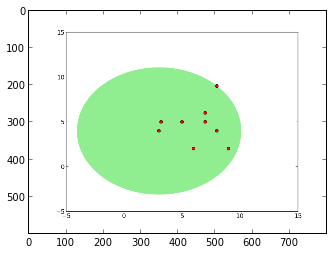
\includegraphics[width=0.7\textwidth]{knn2_files/knn2_fig_04.png}
\par
\end{center}
\end{codeoutput}
\end{codecell}
\begin{codecell}
\begin{codeinput}
\begin{lstlisting}
im=imread("knn1.png");imshow(im)

\end{lstlisting}
\end{codeinput}
\begin{codeoutput}
\begin{verbatim}
<matplotlib.image.AxesImage at 0xc9e166c>
\end{verbatim}
\begin{center}
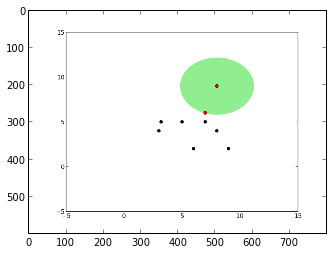
\includegraphics[width=0.7\textwidth]{knn2_files/knn2_fig_05.png}
\par
\end{center}
\end{codeoutput}
\end{codecell}
\begin{codecell}
\begin{codeinput}
\begin{lstlisting}
im=imread("knn2.png");imshow(im)

\end{lstlisting}
\end{codeinput}
\begin{codeoutput}
\begin{verbatim}
<matplotlib.image.AxesImage at 0xcb5b1ac>
\end{verbatim}
\begin{center}
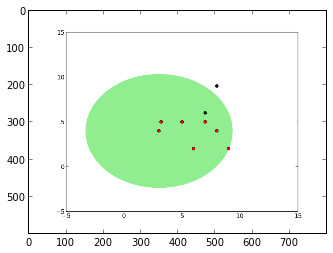
\includegraphics[width=0.7\textwidth]{knn2_files/knn2_fig_06.png}
\par
\end{center}
\end{codeoutput}
\end{codecell}
\begin{codecell}
\begin{codeinput}
\begin{lstlisting}
im=imread("knn3.png");imshow(im)

\end{lstlisting}
\end{codeinput}
\begin{codeoutput}
\begin{verbatim}
<matplotlib.image.AxesImage at 0xcd0b3ec>
\end{verbatim}
\begin{center}
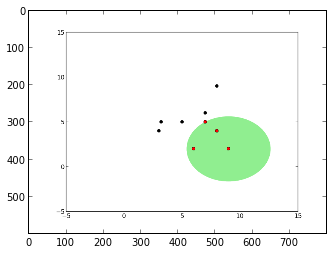
\includegraphics[width=0.7\textwidth]{knn2_files/knn2_fig_07.png}
\par
\end{center}
\end{codeoutput}
\end{codecell}
\begin{codecell}
\begin{codeinput}
\begin{lstlisting}
im=imread("knn4.png");imshow(im)

\end{lstlisting}
\end{codeinput}
\begin{codeoutput}
\begin{verbatim}
<matplotlib.image.AxesImage at 0xce8282c>
\end{verbatim}
\begin{center}
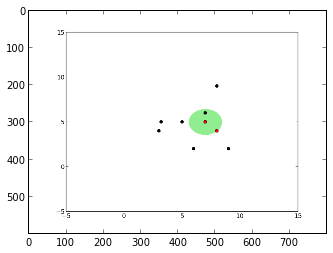
\includegraphics[width=0.7\textwidth]{knn2_files/knn2_fig_08.png}
\par
\end{center}
\end{codeoutput}
\end{codecell}
\begin{codecell}
\begin{codeinput}
\begin{lstlisting}
im=imread("knn5.png");imshow(im)

\end{lstlisting}
\end{codeinput}
\begin{codeoutput}
\begin{verbatim}
<matplotlib.image.AxesImage at 0xcfb836c>
\end{verbatim}
\begin{center}
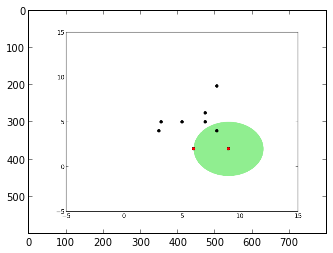
\includegraphics[width=0.7\textwidth]{knn2_files/knn2_fig_09.png}
\par
\end{center}
\end{codeoutput}
\end{codecell}
\begin{codecell}
\begin{codeinput}
\begin{lstlisting}
im=imread("knn6.png");imshow(im)

\end{lstlisting}
\end{codeinput}
\begin{codeoutput}
\begin{verbatim}
<matplotlib.image.AxesImage at 0xd16b58c>
\end{verbatim}
\begin{center}
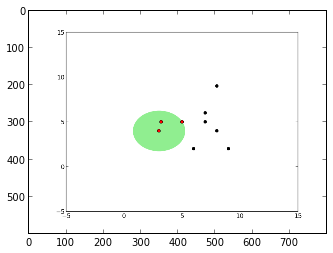
\includegraphics[width=0.7\textwidth]{knn2_files/knn2_fig_10.png}
\par
\end{center}
\end{codeoutput}
\end{codecell}
\begin{codecell}
\begin{codeinput}
\begin{lstlisting}
im=imread("knn7.png");imshow(im)

\end{lstlisting}
\end{codeinput}
\begin{codeoutput}
\begin{verbatim}
<matplotlib.image.AxesImage at 0xd2dfa4c>
\end{verbatim}
\begin{center}
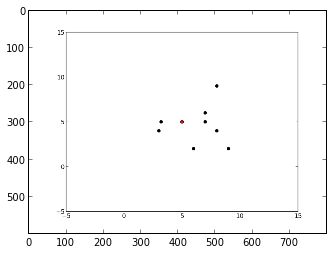
\includegraphics[width=0.7\textwidth]{knn2_files/knn2_fig_11.png}
\par
\end{center}
\end{codeoutput}
\end{codecell}
\begin{codecell}
\begin{codeinput}
\begin{lstlisting}
im=imread("knn8.png");imshow(im)

\end{lstlisting}
\end{codeinput}
\begin{codeoutput}
\begin{verbatim}
<matplotlib.image.AxesImage at 0xd41758c>
\end{verbatim}
\begin{center}
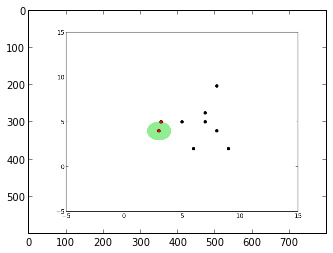
\includegraphics[width=0.7\textwidth]{knn2_files/knn2_fig_12.png}
\par
\end{center}
\end{codeoutput}
\end{codecell}
Kaynaklar, Notlar

{[}1{]} Liu, Moore, Gray, \emph{New Algorithms for Efficient High
Dimensional Non-parametric Classification}

{[}2{]} Alpaydın, \emph{Introduction to Machine Learning}

{[}3{]} Silme islemi ornek kodumuzda Python del ile gerceklestirildi.
Eger bu islem de hizlandirilmak istenirse, en alt kure seviyesindeki
veriler bir oncelik kuyrugu (priority queue) uzerinde tutulabilir, ve
silme islemi hep en sondaki elemani siler, ekleme islemi ise yeni
elemani (hep sirali olan) listede dogru yere koyar.

\end{document}
